\documentclass{beamer}

\usepackage{amsmath}
\usepackage{graphicx}
\usepackage{hyperref}
\usepackage{listings}
\usepackage{color}

\title{Lecture: Introduction to Machine Learning}
\author{KTH AI Student}
\date{\today}

\lstset{
    language=Python,
    basicstyle=\ttfamily\footnotesize,
    keywordstyle=\color{blue},
    stringstyle=\color{red},
    commentstyle=\color{green!50!black},
    breaklines=true,
    showstringspaces=false,
    numbers=left,
    numberstyle=\tiny\color{gray},
    frame=single
}

\begin{document}

\frame{\titlepage}

\section{Introduction to Machine Learning}

\begin{frame}{Introduction}
\begin{itemize}
    \item Machine Learning is a core aspect of modern AI.
    \item Famous for its ability to learn and improve from data without explicit programming.
    \item Goals of this section:
    \begin{itemize}
        \item Understand the basics of Machine Learning.
        \item Explore its types and applications.
    \end{itemize}
\end{itemize}
\end{frame}

\begin{frame}{What is Machine Learning?}
\begin{itemize}
    \item \textbf{Definition:} Machine Learning (ML) is a subfield of Artificial Intelligence (AI) that enables systems to learn and improve from experience.
    \item \textbf{Core Idea:} Use data to make predictions or decisions.
    \item \textbf{Applications:}
    \begin{itemize}
        \item Predicting house prices.
        \item Detecting spam emails.
        \item Recommending products.
    \end{itemize}
\end{itemize}
\begin{figure}
    \centering
    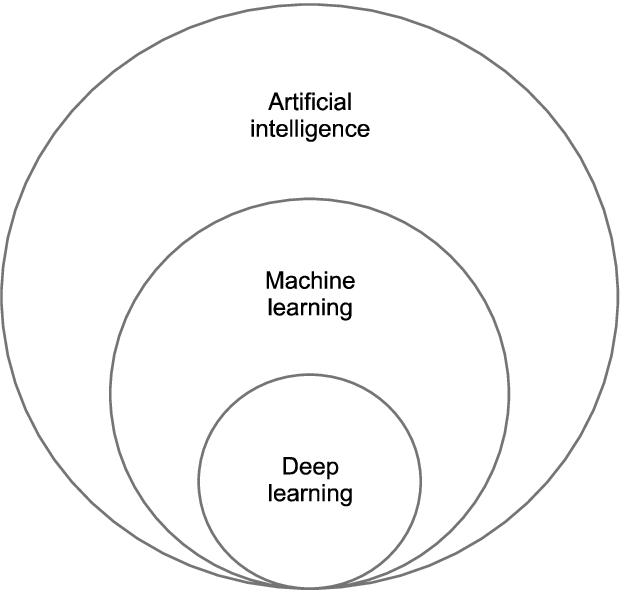
\includegraphics[width=0.4\linewidth]{imgs/ML.png}
    \caption{Machine Learning}
\end{figure}
\end{frame}


\begin{frame}{Types of Machine Learning - Overview}
\begin{itemize}
    \item Machine Learning can be broadly categorized into three types:
    \begin{itemize}
        \item Supervised Learning.
        \item Unsupervised Learning.
        \item Reinforcement Learning.
    \end{itemize}
\end{itemize}
\end{frame}

\begin{frame}{Supervised Learning}
\begin{itemize}
    \item Learns from labeled data.
    \item Examples:
    \begin{itemize}
        \item Classification: Predicting if an email is spam or not.
        \item Regression: Predicting house prices.
    \end{itemize}
    \item Key formula: $y = f(X)$, where $X$ are inputs, and $y$ are outputs.
\end{itemize}
\end{frame}

\begin{frame}{Unsupervised Learning}
\begin{itemize}
    \item Learns from unlabeled data.
    \item Example: Grouping customers based on purchasing behavior.
    \item Focuses on finding patterns and structures in data.
\end{itemize}
\end{frame}

\begin{frame}{Reinforcement Learning}
\begin{itemize}
    \item Learns by interacting with the environment.
    \item Receives rewards for correct actions and penalties for incorrect ones.
    \item Example: Teaching a robot to walk.
\end{itemize}
\end{frame}

\section{Task 1: Data Preprocessing}

\begin{frame}{Data Preprocessing Overview}
\begin{itemize}
    \item Essential step before training ML models.
    \item Tasks:
    \begin{itemize}
        \item Load and clean data.
        \item Handle missing values and categorical variables.
        \item Normalize and split data into training and test sets.
    \end{itemize}
    \item Example Dataset: Heart Disease dataset.
\end{itemize}
\end{frame}

\begin{frame}[fragile]{Steps in Data Preprocessing (Part 1)}
\begin{itemize}
    \item \textbf{Loading Data:} Use pandas to load datasets.
    \item \textbf{Handling Missing Values:} Remove or fill missing entries.
\end{itemize}
\begin{lstlisting}
import pandas as pd

# Load dataset
data = pd.read_csv('heart_disease.csv')

# Display first few rows
print(data.head())
\end{lstlisting}
\end{frame}

\begin{frame}[fragile]{Steps in Data Preprocessing (Part 2)}
\begin{itemize}
    \item \textbf{Encoding Categorical Variables:} Convert categories to numerical values.
    \item \textbf{Splitting Data:} Divide into training and test sets, typically 80-20 split. We divide them to prevent overfitting.
\end{itemize}
\begin{lstlisting}
from sklearn.model_selection import train_test_split
from sklearn.preprocessing import LabelEncoder

# Encode categorical variables
label_encoder = LabelEncoder()
data['category'] = label_encoder.fit_transform(data['category'])

# Split data
X = data.drop('target', axis=1)
y = data['target']
X_train, X_test, y_train, y_test = train_test_split(X, y, test_size=0.2, random_state=42)
\end{lstlisting}
\end{frame}

\begin{frame}{Overfitting and Underfitting}
\begin{itemize}
    \item \textbf{Overfitting:}
    \begin{itemize}
        \item Model learns the training data too well, including noise and outliers.
        \item High accuracy on training data but poor generalization to new data.
        \item Prevention:
        \begin{itemize}
            \item Use simpler models.
            \item Apply regularization techniques (e.g., L1, L2 regularization).
            \item Use cross-validation to tune hyperparameters.
        \end{itemize}
    \end{itemize}
    \item \textbf{Underfitting:}
    \begin{itemize}
        \item Model is too simple to capture the underlying patterns in the data.
        \item Poor performance on both training and test data.
        \item Prevention:
        \begin{itemize}
            \item Use more complex models.
            \item Increase the number of features or use feature engineering.
            \item Reduce regularization.
        \end{itemize}
    \end{itemize}
\end{itemize}
\end{frame}

\begin{frame}[fragile]{Advanced Preprocessing}
\begin{itemize}
    \item Normalize the data to improve model performance:
    \begin{itemize}
        \item StandardScaler: Standardize features by removing the mean and scaling to unit variance.
    \end{itemize}
    \item Feature Engineering:
    \begin{itemize}
        \item Create new features by combining existing ones.
        \item Example: Derive BMI from weight and height.
    \end{itemize}
\end{itemize}
\begin{lstlisting}
from sklearn.preprocessing import StandardScaler

# Normalize data
scaler = StandardScaler()
X_train = scaler.fit_transform(X_train)
X_test = scaler.transform(X_test)

# Feature engineering example
data['BMI'] = data['weight'] / (data['height'] / 100) ** 2
\end{lstlisting}
\end{frame}

\section{Task 2: Training a Classification Model}

\begin{frame}[fragile]{Training a Simple Model: Perceptron}
\begin{itemize}
    \item \textbf{Perceptron:} Basic classification model.
    \item \textbf{Key Steps:}
    \begin{itemize}
        \item Initialize model parameters.
        \item Train model by updating weights.
        \item Evaluate model accuracy on test data.
    \end{itemize}
\end{itemize}
\begin{lstlisting}
from sklearn.linear_model import Perceptron
from sklearn.metrics import accuracy_score

# Initialize and train model
model = Perceptron()
model.fit(X_train, y_train)

# Predict and evaluate
y_pred = model.predict(X_test)
accuracy = accuracy_score(y_test, y_pred)
print(f'Accuracy: {accuracy}')
\end{lstlisting}
\end{frame}

\begin{frame}{Perceptron Visualization}
\begin{itemize}
    \item Example of decision boundary plot.
    \item Helps in understanding how the model separates classes.
\end{itemize}
\begin{figure}
    \centering
    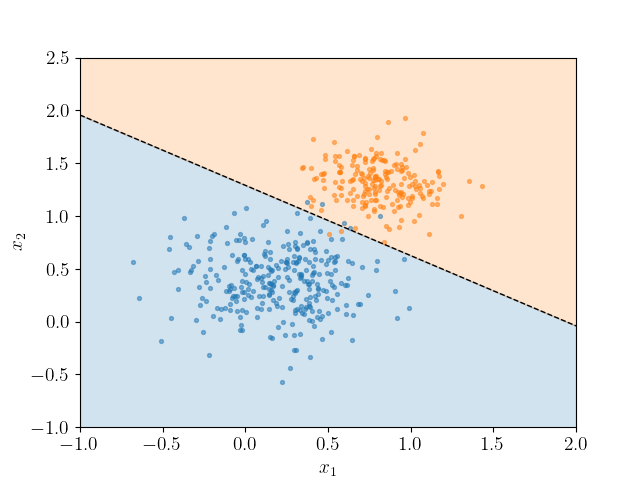
\includegraphics[width=0.8\linewidth]{imgs/perceptron_decision_boundary.png}
    \caption{Decision Boundary of Perceptron Model}
\end{figure}
\end{frame}

\begin{frame}[fragile]{Advanced Classification Models (Part 1)}
\begin{itemize}
    \item Test various models using scikit-learn:
    \begin{itemize}
        \item Logistic Regression.
        \item Support Vector Machines.
    \end{itemize}
\end{itemize}
\begin{lstlisting}
from sklearn.linear_model import LogisticRegression
from sklearn.svm import SVC

# Logistic Regression
log_reg = LogisticRegression()
log_reg.fit(X_train, y_train)
log_reg_pred = log_reg.predict(X_test)

# Support Vector Machine
svm = SVC()
svm.fit(X_train, y_train)
svm_pred = svm.predict(X_test)
\end{lstlisting}
\end{frame}

\begin{frame}[fragile]{Advanced Classification Models (Part 2)}
\begin{itemize}
    \item Test more advanced models:
    \begin{itemize}
        \item Decision Trees.
        \item Random Forests.
    \end{itemize}
\end{itemize}
\begin{lstlisting}
from sklearn.tree import DecisionTreeClassifier
from sklearn.ensemble import RandomForestClassifier

# Decision Tree
tree = DecisionTreeClassifier()
tree.fit(X_train, y_train)
tree_pred = tree.predict(X_test)

# Random Forest
forest = RandomForestClassifier()
forest.fit(X_train, y_train)
forest_pred = forest.predict(X_test)
\end{lstlisting}
\end{frame}

\begin{frame}[fragile]{Evaluation Metrics for Classification}
\begin{itemize}
    \item Metrics to evaluate model performance:
    \begin{itemize}
        \item Accuracy: $\frac{\text{Correct Predictions}}{\text{Total Predictions}}$.
        \item Precision: $\frac{\text{True Positives}}{\text{True Positives + False Positives}}$.
        \item Recall: $\frac{\text{True Positives}}{\text{True Positives + False Negatives}}$.
        \item F1-score: $2 \times \frac{\text{Precision} \times \text{Recall}}{\text{Precision + Recall}}$.
    \end{itemize}
\end{itemize}
\begin{lstlisting}
from sklearn.metrics import precision_score, recall_score, f1_score

# Calculate metrics
precision = precision_score(y_test, y_pred)
recall = recall_score(y_test, y_pred)
f1 = f1_score(y_test, y_pred)

print(f'Precision: {precision}')
print(f'Recall: {recall}')
print(f'F1 Score: {f1}')
\end{lstlisting}
\end{frame}

\section{Task 3: Best Practices and Hyperparameter Tuning}

\begin{frame}{Model Evaluation Metrics}
\begin{itemize}
    \item \textbf{Accuracy:} Proportion of correct predictions.
    \item \textbf{Precision:} Correct positive predictions out of total predicted positives.
    \item \textbf{Recall:} Correct positive predictions out of actual positives.
    \item \textbf{F1-Score:} Harmonic mean of precision and recall.
\end{itemize}
\end{frame}

\begin{frame}{What is a Hyperparameter?}
\begin{itemize}
    \item \textbf{Definition:} Hyperparameters are parameters whose values are set before the learning process begins.
    \item \textbf{Examples:}
    \begin{itemize}
        \item Learning rate in gradient descent.
        \item Number of trees in a random forest.
        \item Number of clusters in K-Means.
    \end{itemize}
    \item \textbf{Importance:}
    \begin{itemize}
        \item They control the training process and model complexity.
        \item Proper tuning can significantly improve model performance.
    \end{itemize}
\end{itemize}
\end{frame}

\begin{frame}[fragile]{Hyperparameter Tuning}
\begin{itemize}
    \item \textbf{Grid Search:} Explore combinations of parameters to find the best configuration.
    \item \textbf{Cross-Validation:} Evaluate model on different data splits to ensure reliability.
\end{itemize}
\begin{lstlisting}
from sklearn.model_selection import GridSearchCV

# Define parameter grid
param_grid = {
    'C': [0.1, 1, 10],
    'kernel': ['linear', 'rbf']
}

# Initialize Grid Search
grid_search = GridSearchCV(SVC(), param_grid, cv=5)
grid_search.fit(X_train, y_train)

# Best parameters
print(f'Best Parameters: {grid_search.best_params_}')
\end{lstlisting}
\end{frame}

\section{Task 4: Regression Models}

\begin{frame}{Overview of Regression Models}
\begin{itemize}
    \item Examples of models:
    \begin{itemize}
        \item Linear Regression.
        \item Support Vector Machines for Regression.
        \item Decision Trees.
        \item Random Forests.
    \end{itemize}
\end{itemize}
\end{frame}

\begin{frame}[fragile]{Evaluating Regression Models}
\begin{itemize}
    \item Metrics to assess model performance:
    \begin{itemize}
        \item Mean Squared Error. $MSE=\frac{1}{n} \sum_{i=1}^{n} (y_i - \hat{y}_i)^2$.
        \item Coefficient of Determination. $R^2 = 1 - \frac{\sum_{i=1}^{n} (y_i - \hat{y}_i)^2}{\sum_{i=1}^{n} (y_i - \bar{y})^2}$.
    \end{itemize}
\end{itemize}
\begin{lstlisting}
from sklearn.metrics import mean_squared_error, r2_score

# Calculate metrics
mse = mean_squared_error(y_test, y_pred)
r2 = r2_score(y_test, y_pred)

print(f'Mean Squared Error: {mse}')
print(f'R^2 Score: {r2}')
\end{lstlisting}
\end{frame}

\begin{frame}{Visualizing Regression Results}
\begin{itemize}
    \item Compare predicted values against true values.
    \item Use scatter plots for analysis.
\end{itemize}
\begin{figure}
    \centering
    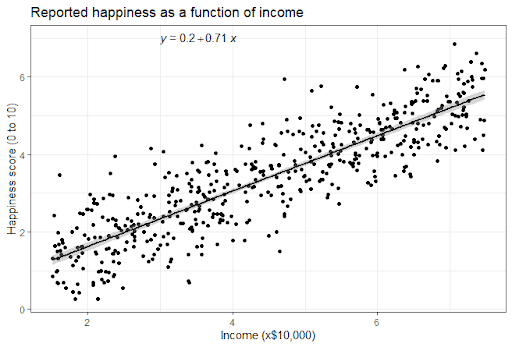
\includegraphics[width=0.8\linewidth]{imgs/regression_results.png}
    \caption{Regression Results Visualization}
\end{figure}
\end{frame}

\section{Task 5: Clustering}

\begin{frame}{Introduction to Clustering}
\begin{itemize}
    \item \textbf{Definition:} Group similar data points based on features.
    \item \textbf{Applications:}
    \begin{itemize}
        \item Customer segmentation.
        \item Image segmentation.
    \end{itemize}
\end{itemize}
\end{frame}

\begin{frame}[fragile]{Examples of Clustering Algorithms}
\begin{itemize}
    \item Common algorithms:
    \begin{itemize}
        \item K-Means.
        \item DBSCAN.
        \item Agglomerative Clustering.
        \item Gaussian Mixture Models.
    \end{itemize}
\end{itemize}
\begin{lstlisting}
from sklearn.cluster import KMeans

# Initialize and fit K-Means
kmeans = KMeans(n_clusters=3)
kmeans.fit(X)

# Predict clusters
clusters = kmeans.predict(X)

# Cluster centers
centers = kmeans.cluster_centers_
\end{lstlisting}
\end{frame}

\begin{frame}{Visualizing Clusters}
\begin{itemize}
    \item Plot clusters using scatter plots with different colors.
    \item Analyze cluster characteristics and separability.
\end{itemize}
\begin{figure}
    \centering
    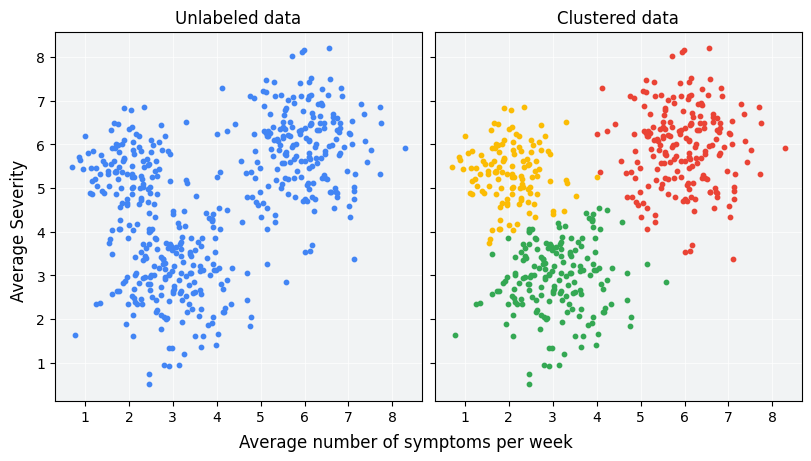
\includegraphics[width=0.8\linewidth]{imgs/clusters.png}
    \caption{Cluster Visualization}
\end{figure}
\end{frame}

\section{Conclusion}

\begin{frame}{Summary}
\begin{itemize}
    \item Recap of all tasks and key concepts:
    \begin{itemize}
        \item Introduction to Machine Learning.
        \item Data preprocessing steps.
        \item Training and evaluating classification and regression models.
        \item Clustering and its applications.
    \end{itemize}
    \item Importance of proper evaluation and tuning in ML pipelines.
\end{itemize}
\end{frame}

\begin{frame}{Resources}
    \begin{figure}
        \centering
        \begin{minipage}{0.45\linewidth}
            \centering
            
\includegraphics[width=\linewidth]{imgs/pytorch.jpg}
            \caption{This one good for code + basic theory}
        \end{minipage}
        \hfill
        \begin{minipage}{0.45\linewidth}
            \centering
            
\includegraphics[width=\linewidth]{imgs/ml.jpg}
            \caption{This one good for theory}
        \end{minipage}
    \end{figure}
\end{frame}

\begin{frame}{Resources}
\begin{figure}
    \centering
    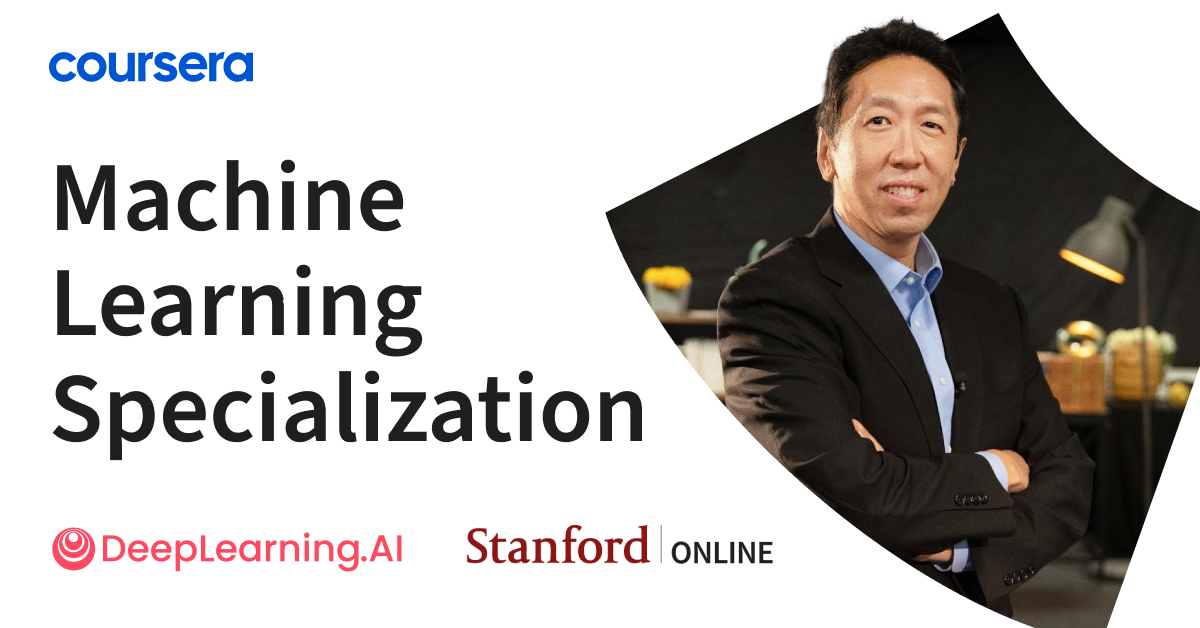
\includegraphics[width=0.8\linewidth]{imgs/andrew_ng.png}
    \caption{You can get the certification for free if you say you are a student}
\end{figure}
\end{frame}

\begin{frame}{Resources}
    You can also take the following courses at KTH:
    \begin{itemize}
        \item \textbf{Foundations of Machine Learning (DD1420)}: Introduces the basic principles and algorithms in machine learning.
        \item \textbf{Artificial Intelligence (DD2380)}: Covers fundamental AI concepts and techniques.
        \item \textbf{Machine Learning, Advanced Course (DD2434)}: Delves deeper into advanced machine learning methodologies and applications.
        \item \textbf{Deep Learning in Data Science (DD2424)}: Focuses on deep learning techniques for data science, emphasizing neural networks and large-scale data analysis.
        \item \textbf{Artificial Neural Networks and Deep Architectures (DD2437)}: Provides an in-depth understanding of neural network architectures and training methods.
    \end{itemize}
\end{frame}


\end{document}